\documentclass{ctexart}
\usepackage{amsmath}
\usepackage{amsfonts}
\usepackage{amssymb}
\usepackage{graphicx}
\usepackage{longtable}
\usepackage{CJK}
\usepackage{float}
\usepackage{cases}
\usepackage{array}

\newcommand{\PreserveBackslash}[1]{\let\temp=\\#1\let\\=\temp}
\newcolumntype{C}[1]{>{\PreserveBackslash\centering}p{#1}}
\newcolumntype{R}[1]{>{\PreserveBackslash\raggedleft}p{#1}}
\newcolumntype{L}[1]{>{\PreserveBackslash\raggedright}p{#1}}
\newtheorem{define}{\hspace{2em}推导}
\usepackage{supertabular}
\setlength{\LTcapwidth}{6cm} 
\author{吴秉哲}
\title{数值分析上机报告}
\begin{document}
\maketitle
这学期每次的上机报告都按如下格式编写:

每份报告分为几个章节,每个章节分别介绍上机作业中的一题,其中每个
章节又分为以下几个部分:
\begin{enumerate}
\item 问题提出及相关背景知识
\item 问题的理论分析及解决方案
\item 程序的部分设计思路与细节
\item 计算成果与分析
\item 本次上机的反思
\end{enumerate}
每个题目中要求回答的问题均蕴含在问题的理论分析与计算成果分析两部分

在程序方面,都是由C++编写完成(其中用到了自己编写的库:矩阵(Matrix),向量(Vector),以及数值代数的相关算法(linear)),在linux下由g++编译。数据方面
一般使用matlab可视化处理,少部分使用了python。
\section{第三章第一题}
\subsection{问题提出及相关背景知识}
题目要求使用数值方法求$f(x)=ln(x)$在$x=0.7$处的微分。并要求对不同的h进行实验,要求观察所得的现象。题目给出的数值格式有三种。
\subsection{问题的理论分析及解决方案}
鉴于题目的形式,我们可以通过f(x)与h的信息,获得可数个点的信息。
于是可以考虑$f(x)$在$x=0.7$处的泰勒展开,然后对不同的等式进行
相加与相减的操作,便可以得到题目的三个数值格式。我们对第三个格式进行详细推导,并在推导过程中给出其截断误差的阶:

当$f(x)$6阶连续可微时,将$f(x)$在x处,分别对$f(x+h),f(x-h),f(x+2h),f(x-2h)$进行
泰勒展开,可得:
\begin{equation*}
f(x+h)=f(x)+hf'(x)+\dfrac{1}{2}h^2f^{(2)}(x)+\dfrac{1}{6}h^3f^{(3)}(x)+\dfrac{1}{24}h^4f^{(4)}(x)+\dfrac{1}{120}h^5f^{(5)}(x)+O(h^6)
\end{equation*}
\begin{equation*}
f(x-h)=f(x)-hf'(x)+\dfrac{1}{2}h^2f^{(2)}(x)-\dfrac{1}{6}h^3f^{(3)}(x)+\dfrac{1}{24}h^4f^{(4)}(x)-\dfrac{1}{120}h^5f^{(5)}(x)+O(h^6)
\end{equation*}
\begin{equation*}
f(x+2h)=f(x)+2hf'(x)+\dfrac{1}{2}(2h)^2f^{(2)}(x)+\dfrac{1}{6}(2h)^3f^{(3)}(x)+\dfrac{1}{24}(2h)^4f^{(4)}(x)+\dfrac{1}{120}(2h)^5f^{(5)}(x)+O(h^6)
\end{equation*}
\begin{equation*}
f(x-2h)=f(x)-2hf'(x)+\dfrac{1}{2}(2h)^2f^{(2)}(x)-\dfrac{1}{6}(2h)^3f^{(3)}(x)+\dfrac{1}{24}(2h)^4f^{(4)}(x)-\dfrac{1}{120}(2h)^5f^{(5)}(x)+O(h^6)
\end{equation*}
则由上面四式可得:
\begin{equation*}
f'(x)=\dfrac{f(x-2h)-8f(x-h)+8f(x+h)-f(x-2h)}{12h}+\dfrac{1}{30}h^4f^{(5)}(x)+O(h^5)
\end{equation*}
上式略去高阶项即可得题目所给的数值格式,并由上式可以看出其截断误差的阶为$O(h^4)$

由上面的推导,可以得出题目所给的第三个数值格式的精度阶远远大于前两个数值格式,从后面的计算结果也可以看出这一点。

此外,题目还给出了另外两种数值格式:
\begin{enumerate}
\item 向前差分格式
\[f'(x)\approx \dfrac{f(x+h)-f(x)}{h}\]
\item
\[f'(x)\approx \dfrac{f(x+h)-f(x-h)}{2h}\]
\end{enumerate}
容易推导上面两种格式的截断误差阶数分别为一阶与二阶。
\subsection{程序的部分设计思路与细节}
本题的程序较为简单,考虑到代码的重复可用写了数值微分的计算函数库,
包含了本题的三种数值格式。在主程序中利用循环给出了$h=1/10^k,k=1,/cdots,10$的数值结果。
\subsection{计算成果与分析}
下面列出三种计算结果(保留5位小数)的表格,包含每种格式的误差,表格如下: 
\begin{center} 
\begin{longtable}{|c|c|c|c|c|c|c|c|}

\caption{上机习题3.1} \\ 
%begin{tabular}{|c|c|c|c|c|c|c|}
\hline 
真实值& h& 向前差分格式& 误差&中心差分格式& 误差& 4阶精度格式& 误差 \\
\hline
1.4286& $1/10^1$& 1.3353& 0.093258& 1.4384& 0.0098389& 1.4281& 0.00051317\\
\hline
1.4286& $1/10^2$& 1.4185& 0.010108& 1.4287& 9.7194e-05& 1.4286& 4.7634e-08\\
\hline
1.4286& $1/10^3$& 1.4276& 0.0010194& 1.4286& 9.7182e-07& 1.4286& 4.7198e-12\\
\hline
1.4286& $1/10^4$& 1.4285& 0.00010203& 1.4286& 9.718e-09& 1.4286& 3.1619e-13\\
\hline
1.4286& $1/10^5$& 1.4286& 1.0204e-05& 1.4286& 9.1832e-11& 1.4286& 6.2375e-12\\
\hline
1.4286& $1/10^6$& 1.4286& 1.0204e-06& 1.4286& 2.5219e-11& 1.4286& 5.2975e-11\\
\hline
1.4286& $1/10^7$& 1.4286& 1.0289e-07& 1.4286& 7.5194e-10& 1.4286& 9.3697e-10\\
\hline
1.4286& $1/10^8$& 1.4286& 7.5194e-10& 1.4286& 7.5747e-09& 1.4286& 1.1738e-08\\
\hline
1.4286& $1/10^9$& 1.4286& 5.6263e-08& 1.4286& 5.6263e-08& 1.4286& 8.8645e-08\\
\hline
1.4286& $1/10^{10}$& 1.4286& 2.768e-07& 1.4286& 2.768e-07& 1.4286& 4.6184e-07\\
\hline
\end{longtable}
\end{center} 

由上面的计算结果,可以得到如下几条信息:
\begin{enumerate}
\item 
从上表可以看出题目中的第三种数值格式(4阶精度)在$h=1/10^{3}$的时候误差已经减小到$10^{-12}$,效果远远好于前两种格式,另外,中心差分的效果好于向前差分格式,这与我们的理论推导想吻合(向前差分为一阶,中心差分为二阶,第三种数值格式为四阶)
\item
从上表可以发现一个现象:三种数值格式的计算结果在h小于某个值的时候都会出现误差增大的情况,为方便,我们将这个值称为临界值,而且容易观察出,截断误差的阶数越大,临界值越大。出现这一现象的原因是因为计算机对浮点数的计算是有舍入误差的,下面只举向前差分格式进行说明(其余两种格式类似):
设$f(x+h)$与$f(x)$分别有舍入误差$\varepsilon_1$与$\varepsilon_2$,记$\varepsilon=max\{|\varepsilon_1|,|\varepsilon_2|\}$,从而函数值为:
\[\overline{f}(x+h)=f(x+h)+\varepsilon_1,\overline{f}(x)=f(x)+\varepsilon_2\]
我们在用向前差分公式来计算$f'(x)$时,不妨就使用$f'(x)$表示数值解,即有:
\[f'(x)=\dfrac{f(x+h)-f(x)}{h},\overline{f'}(x)=\dfrac{\overline{f}(x+h)-\overline{f}(x)}{h}\]
在此,我们忽略h的舍入误差.由此即可得数据的舍入误差带来的计算结果误差为:
\[\delta(f'(x))=|f'(x)-\overline{f'}(x)|\leq \dfrac{|\varepsilon_1|+|\varepsilon_2|}{h}\leq \dfrac{2\varepsilon}{h}\]
由此可见,h越小,已知数据的舍入误差就可能被放得更大!考虑截断误差与
舍入误差的总和,可以用求极值的方法求到上面所提到的临界值,在这里不详细推导了。由上面的推导,我们不难解释上面计算结果出现如此现象的原因了。
\end{enumerate}
\subsection{本次上机的反思}
通过对本题的三种数值微分格式进行实验,我总结了如下的经验:
\begin{enumerate}
\item 通过计算结果分析这一部分的对误差的推导,我们在实际计算中不应该将h
取得太小,不然误差反而会增加
\item 
显示的数值微分格式都是数值不稳定的,这由h小于某个值后,随着h的减小,误差反而增大可以看出。所以我们在实际计算中应该尽量使用数值稳定性较好的隐式数值微分格式,这样可以避免本题计算中出现的这一问题。
\item 
在实际编制程序之前,应该对问题的数值算法有个理论的误差分析,这样可以选择合适的方法及数据进行计算,否者,可能会出现本题类似于h取得太小而影响结果的情况。
\end{enumerate}
\section{第三章第二题}
\subsection{问题提出及相关背景知识}
题目要求分别使用显示中心格式与隐式格式计算$f(x)=\exp(-\dfrac{x}{4}),0\leq x \leq 1$的数值微分,并将计算结果与精确值比较。其中题目要求,区间[0,1]十等分。
\subsection{问题的理论分析及解决方案}
我们在这里推导题目所要求的两种数值微分格式。设$x_i,i=0,1,\cdots,n-1$为题目的节点,其中$n=11$。设$f(x)=\exp(-\dfrac{x}{4})$,容易
看出$f(x)$无穷次可微,利用Taylor展开公式有:
\begin{equation} f(x_{i+1})=f(x_i)+hf'(x_i)+\cdots+\dfrac{h^k}{k!}f^{(k)}(\xi_1),
\end{equation} 
\begin{equation} f(x_{i-1})=f(x_i)-hf'(x_i)+\cdots+\dfrac{(-h)^{k}}{k!}f^{(k)}(\xi_2)\end{equation}
其中$\xi_1 \in (x_i,x_{i+1}),\xi_2 \in (x_{i-1},x_i)$
在(1),(2)中取$k=3$,并将两式相减可得中心差分格式:
\[f'(x_i)\approx \dfrac{f(x_{i+1})-f(x_{i-1})}{2h}\]
下面简单推导隐式格式,在(1),(2)中取$k=6$两式相加可得:
\begin{equation}
\dfrac{f(x_w{i+1})-2f(x_i)+f(x_{i-1})}{h^2}=f''(x_i)+\dfrac{1}{12}h^2f^{(4)}(x_i)+O(h^4)
\end{equation}
在(1),(2)中取$k=7$,两式相减可得
\begin{equation}
f'(x_i)=\dfrac{f(x_{i+1})-f(x_{i-1})}{2h}-\dfrac{h^2}{6}f'''(x_i)-\dfrac{h^4}{120}f^{(5)}(x_i)+O(h^4)
\end{equation}
由(3)式可得:
\[f'''(x_i)=\dfrac{f'(x_{i+1})-df'(x_i)+f'(x_{i-1})}{h^2}-\dfrac{1}{12}h^2f^{(5)}(x_i)+O(h^4)\]
将此式代入(4)式,略去其中$O(h^4)$的项,对$i=0,1,\cdots,n-1$记$f'(x_i)$的近似值为$m_i$,并记$f(x_i)=f_i$,则有:
\[ m_i=\dfrac{f_{i+1}-f_{i-1}}{2h}-\dfrac{1}{6}(m_{i+1}-2m_i+m_{i-1}),i=1,2,\cdots,n-1.\]
再补充两个边界条件,例如假设$f'(x_0),f'(x_n)$已知,则可以得到一个关于$m_i$的线性方程组:
$$\left\{\begin{aligned}
& m_{i-1}+4m_i+m_{i+1}=\dfrac{3}{h}(f_{i+1}+f_{i-1}),&i=1,2\cdots,n-1, \\
& m_0=f'(x_0),m_n=f'(x_n)
\end{aligned}
\right.
$$
这是一个系数矩阵为三对角的矩阵,可以使用追赶法快速求解。解出来的$m_i$即为要求的数值解。上述便是数值微分的隐式格式
\subsection{程序的部分设计思路与细节}
中心差分显示格式的程序比较容易实现。隐式格式需要用追赶法求解三对角方程,而程序涉及到对边界条件的处理,需要仔细检查程序中边界条件部分的实现,不然会出现程序的逻辑错误。
\subsection {计算成果与分析}
下面先列出两种方法得出的结果(double环境下),然后对结果进行对比分析:
\begin{center}
\begin{longtable}{|c|c|cc|cc|}
\caption{习题3.2}\\
\hline
i& 精确值& 中心差商格式 & 误差& 隐式格式 & 误差 \\
\hline
0.1& -0.24383& -0.24385& 2.5399e-05& -0.24383& 6.7446e-10  \\
\hline
0.2& -0.23781& -0.23783& 2.4772e-05& -0.23781& 4.7708e-10 \\
\hline
0.3& -0.23194& -0.23196& 2.4161e-05& -0.23194& 5.1377e-10 \\
\hline
0.4& -0.22621& -0.22623& 2.3564e-05& -0.22621& 4.8792e-10 \\
\hline
0.5& -0.22062& -0.22065& 2.2982e-05& -0.22062& 4.8008e-10 \\
\hline
0.6& -0.21518& -0.2152& 2.2415e-05& -0.21518& 4.6455e-10 \\
\hline
0.7& -0.20986& -0.20989& 2.1862e-05& -0.20986& 4.6358e-10 \\
\hline
0.8& -0.20468& -0.2047& 2.1322e-05& -0.20468& 4.1381e-10 \\
\hline
0.9& -0.19963& -0.19965& 2.0795e-05& -0.19963& 5.464e-10\\
\hline 
\end{longtable}
\end{center}
由上面的表格很容易看出:中心差分格式的格式的误差在$10^{-5}$量级,隐式格式的误差达到了$10^{-10}$,后者的精度远远高于前者。除了这一点,上述数据还有如下的规律:中心差商格式的误差随着i的增大,误差在不断减小,而隐式格式的误差和i的增长并没有什么直接关系,这一点的原因其实不难推断,隐式格式是一下解方程解出所有要求的值,而中心差商公式是一项项求得。

最后,进一步实验,不断减小h的值,即加细区间的划分,可以看到随着n
的增大,隐式格式的误差变小得越来越快,而中心格式误差的速度相对缓慢。有这些计算结果猜测当n增大到一个值后,误差的量级将不会变化,而隐式格式的误差会随着n的增大,趋向于0。这也进一步说明了隐式格式的数值稳定性好。
\subsection{本次上机的反思}
通过本题的实验有如下的收获:
\begin{enumerate}
\item 
相对于中心差商格式,隐式格式可以通过解一个三对角的线性方程组一下求出所有节点的数值微分,而且精度很高,数值稳定性好,在以后
求解实际问题的时候应该尽量选择这种方法。
\item 
在一开始编写隐式格式的时候,处理边界条件不够小心,出现了程序的逻辑错误,以后在处理类似的问题的时候,一定要
事先想清楚条件,这样可以提高编写程序的效率。
\end{enumerate}
\section{第三章第四题}
\subsection{问题提出及相关背景知识}
本题要求分别运用不同的数值积分算法对积分$\int_{0}^{1}\dfrac{4}{1+x^2}$计算,由此可以得到不同精度的$\pi$值
\subsection{问题的理论分析及解决方案}
对于数值积分可以采用常规的复合中点公式,复合梯形公式和复合Simpson公式求解。这三种方法实现及理论推导较为简单,在这里不再
推导。下面主要引入Romberg公式与自适应求积方法。

首先简单推导一下Romberg公式。Romberg公式是通过将Richardson外推加速收敛技术应用于复合梯形求积公式得到的一种
数值积分的方法。为此,先介绍这种加速收敛技术。
\begin{define}
(Richardson加速收敛技术)假设我们要用一个与步长h有关的量$Q_1(h)$去近似一个与h无关的量Q,而且知道截断误差的渐近展开式为:
\[Q-Q_1(h)=c_1h^{p_1}+c_2h^{p_2}+\cdots+\]
其中$c_k,p_k$为常数,且$p_k$按升序排列,此时$Q_1$逼近Q的截断误差量级就为$O(h^{p_1})$

如果我们将步长缩小一倍,即取$h=h/2$,则有
\begin{equation*}
\begin{split}
Q-Q_1(h/2) &=c_1(h/2)^{p_1}+c_2(h/2)^{p_2}\cdots \\
 &=2^{-p_1}c_1h^{p_1}+2^{-p_2}c_2h^{p_2}+\cdots
\end{split}
\end{equation*}
把前式乘上$2^{-p_1}$再减去上式,整理可得:
\[Q-\dfrac{Q_1(h/2)-2^{-p_1}Q_1(h)}{1-2^{-p_1}}=c_2^*h^{p_2}+c_3^{*}h^{p_3}+\cdots \]
其中常数$c_k^{*}$为:
\[c_k^{*}=\dfrac{c_k(2^{-p_k}-2^{-p_1})}{1-2^{-p_1}}\]
记:
\[Q_2(h)=\dfrac{Q_1(h/2)-2^{-p_1}Q_1(h)}{1-2^{-p_1}}\]
则由上面规则继续下去可以得到$Q_{i}(h)$,其截断误差为$O(h^p_i)$上述这种方法称为Richardson外推加速收敛技术。
\end{define}
将上述的技术运用到复合梯形求积公式,就可以得到Romberg公式。具体做法如下:
\begin{define}
(Romberg求积)当$f$充分光滑时,可以得到梯形公式的截断误差渐进展开式:
\[\int_{a}^{b}f(x)dx=T_1(h)+\sum_{k=1}^{\infty}c_{2k}^{(1)}h^{2k}\]
其中 $c_{2k}^{(1)}$为常数,
\[T_2(h)=\dfrac{T_1(h)-4^{-1}T_1(h)}{1-4^{-2}}\]
根据上述的截断误差式,我们可以推出一般的求积序列:
\[T_{k+1}(h)=\dfrac{T_k(h/2)-4^{-k}T_k(h)}{1-4^{-k}}\]
并可以得到:
\[\int_a^bf(x)dx-T_{k+1}(h)=O(h^{2(k+1)})\]
\end{define}
上述即为Romberg公式。下面简单介绍自适应求积方法(以复合梯形公式为例)
\begin{define}
(自适应求积方法)记$T_n$为n等分$[a,b]$后由复合梯形求积公式所求得的积分值,
于是$T_n=\dfrac{h}{2}\sum\limits_{k=0}^{n-1}[f(x_k)+f(x_{k+1})]$,将$[a,b]$ $2n$等分后,n等分下的子区间$[x_k,x_{k+1}]$变为两个
更小的区间$[x_k,x_{k+1/2}],[x_{k+1/2},x_{k+1}]$,从而可以得到
\[
T_{2n}=\dfrac{1}{2}T_n+\dfrac{h}{2}\sum_{k=0}^{n-1}f(x
_{k+1/2})
\]
\end{define}
这样就可以先将区间分得粗糙一些,然后根据所要精度不断调整,这种方法的好处是减少计算机舍入误差对梯形公式的影响。

\subsection{程序的部分设计思路与细节}
本次的程序根据算法很容易实现。其中Romberg算法需要编制一个复合梯形求积公式,并不断折半初始步长$h$,在这次作业中,我直接使用了递归来实现,编出来的程序十分简洁。
\subsection{计算成果与分析}
下面列出本次上机程序的计算结果。(取$\pi\approx3.1415926589793$与计算结果进行对比)

首先我们来对比未用任何其他技术的数值积分格式的结果(复合中点,复合梯形,复合Simposon)(由于篇幅只列出一部分,其余一些特殊的现象用文字描述):
\begin{center}
\begin{longtable}{|c|c|cc|}
\caption{3.4复合中点公式计算结果}\\
\hline
h& $\pi$& 复合中点& 误差\\
\hline
1& 3.141593& 3.2& 0.05840735\\
\hline
0.1& 3.141593& 3.142426& 0.0008333314\\
\hline
0.01& 3.141593& 3.141601& 8.333333e-06\\
\hline
0.001& 3.141593& 3.141593& 8.333334e-08\\
\hline
0.0001& 3.141593& 3.141593& 8.333352e-10\\
\hline
1e-05& 3.141593& 3.141573& 2.000009e-05\\
\hline
1e-06& 3.141593& 3.141593& 3.508305e-14\\
\hline
\end{longtable}
\begin{longtable}{|c|c|cc|}
\caption{3.4复合梯形公式}\\
\hline
h& $\pi$& 复合梯形& 误差\\
\hline
1& 3.141593& 3& 0.1415927\\
\hline
0.1& 3.141593& 3.139926& 0.001666665\\
\hline
0.01& 3.141593& 3.141576& 1.666667e-05\\
\hline
0.001& 3.141593& 3.141592& 1.666667e-07\\
\hline
0.0001& 3.141593& 3.141593& 1.666679e-09\\
\hline
1e-05& 3.141593& 3.141573& 2.000012e-05\\
\hline
1e-06& 3.141593& 3.141593& 2.176037e-13\\
\hline
\end{longtable}
\begin{longtable}{|c|c|cc|}
\caption{3.4复合Simpson}\\
\hline
h& $\pi$& 复合Simposon& 误差\\
\hline
1& 3.141593& 3.133333& 0.00825932\\
\hline
0.1& 3.141593& 3.141593& 6.20008e-10\\
\hline
0.01& 3.141593& 3.141593& 2.664535e-15\\
\hline
0.001& 3.141593& 3.141593& 2.220446e-15\\
\hline
0.0001& 3.141593& 3.141593& 2.220446e-15\\
\hline
1e-05& 3.141593& 3.141573& 2.00001e-05\\
\hline
1e-06& 3.141593& 3.141593& 4.92939e-14\\
\hline
\end{longtable}
\end{center}
从上面表格可以得出,复合Simpson格式的计算误差远远小于其余两个格式,这也与它们各自的代数精度吻合。仔细观察还可以发现,在用复合Simposon公式计算的时候,当$h=0.01$的时候,已经接近机器精度,但是随着$h$的减小,误差反而有变大的趋势,通过实验发现另外两个公式的计算结果也有如此的现象,这样就验证了如下的规律:对于这三种数值积分的格式,都存在某个$h$值,当小于这个值后,再减小这个$h$的值,计算将不再改进。究其原因,是因为舍入误差的存在,当取样点增多时, 每个取样点 的函数值 被 截尾 的部分就增加 了,由于 取样点很多,这个误差就 以取样点的个数为倍放大 , 就导致最终的结果出现比较大 的误差。

下面列出Romberg求积法与自适应求积法的计算结果:
\begin{center}
\begin{longtable}{|c|c|c|}
\caption{3.4Romberg求积法}\\
\hline
误差& 计算结果& Romberg迭代次数\\
\hline
6.2000893e-10& 3.1415927& 2\\
\hline
3.0998315e-11& 3.1415927& 3\\
\hline
0& 3.1415927& 4\\
\hline
1.3322676e-15& 3.1415927& 5\\
\hline
1.7763568e-15& 3.1415927& 6\\
\hline
1.3322676e-15& 3.1415927& 7\\
\hline
\end{longtable}
\end{center}
从上表可以看出使用加速收敛技术后,数值计算的效果特别好,第二次迭代的精度已经达到了$10^{-10}$的,在迭代4次过后,误差已经达到了机器精度,运算的速度相比于前面三种公式已经快了很多,而且由于方法的不同,这种方法也减少了舍入误差对结果的影响(这可以从计算的精度看出)

下面,我们再来看看自适应方法的结果:
\begin{center}
\begin{longtable}{|c|c|c|}
\caption{自适应方法计算结果}\\
\hline
精度& 达到精度步长& 自适应方法调整次数\\
\hline
0.00041666664& 0.05& 2\\
\hline
2.6041667e-05& 0.0125& 4\\
\hline
1.0172526e-07& 0.00078125& 8\\
\hline
1.5894561e-09& 9.765625e-05& 11\\
\hline
2.4825475e-11& 1.2207031e-05& 14\\
\hline
1.1635137e-13& 7.6293945e-07& 18\\
\hline
\end{longtable}
\end{center}
由上表对比复合梯形公式的计算结果可以看出,使用自适应求积方法得到的结果与复合梯形公式得到的结果大致相当,也就是指这两种方法达到相同的精度所需的步长相当。可见自适应方法并没有改变梯形求积公式的实质,它相对于梯形公式的好处是它的程序可以自动调整帮我们达到我们所需要的精度。
\subsection{本次上机的反思}
从上面计算结果分析,Romberg方法计算的结果精度,计算的速度都远远好于其余的方法,所以在对计算结果精度要求比较高的情况下可以使用Romberg求积方法。如果要考虑到计算所耗费的空间,时间可以考虑自适应方法,这样可以根据我们所需要的精度做计算上的相应调整,达到资源的最大化利用。
\section{第三章第六题}
\subsection{问题提出及相关背景知识}
本题要求用数值方法计算$\int_{0}^{+\infty}\dfrac{x^3}{e^x-1}dx$,并比较不同方法的计算效率与精度。本题要求计算的积分具有深刻的物理背景,这积分首先出现在对黑体辐射的能量密度频谱的推导过程中,
下面一部分来介绍本题的两种解法。
\subsection{问题理论分析及解决方案}
其实本题的积分可以有一种避开书上所有数值计算方法的公式,在理论上我们可以证明如下的式子:
\[\int_{0}^{+\infty}\dfrac{x^3}{e^x-1}dx=\dfrac{\pi^4}{15}\]
有了这个等式,我们就可以将此积分转化为对$\pi$的计算,而后者的计算是简单的而且可以达到很高的精度,这样我们就可以将用此种方法计算得到的值近似的作为题目积分的精确值,而题目要求用数值积分方法来计算,所以下面我们着重来设计适合本题的数值积分方法。
\begin{enumerate}
\item 方法一

注意到被积函数随着$x$的增大,衰减得很快,于是我们可以取一个适当大的积分上限,一个适当小的数作为积分下限,然后让这个有穷积分来近似题目中的广义积分,在实际编写程序的过程中,我选取$10^k$作为积分上限,
$10^{-k}$作为积分下限(程序会根据我们对计算精度的需要自动的调整k的大小),然后通过前面的数值积分方法计算$\int\limits_{10^{-k}}^{10^k}$
\item 方法二(Gauss—Laguerre)
高斯-拉盖尔方法是指用如下的公式近似所要求的无穷积分值:
\[\int_{0}^{\infty}e^{-x}f(x)dx\approx \sum_{i=1}^{n}\omega_if(x_i)\]
其中$x_i$是拉盖尔多项式$L_n(x)$的第$i$个根,权值$\omega_i$满足:
\[\omega_i=\dfrac{x_i}{(n+1)^2[L_{n+1}(x_i)]^2}\]
Gauss-Laguerre求积公式的节点$x_i$及求积系数$A_i$见下表。
\begin{center}
\bf{Gauss-Laguerre求积节点和求积系数}
\end{center}
$$
\small\begin{array}{|c|c|c|c|c|c|c|}
\hline
n&x_i&A_i&&n&x_i&A_i\\
\hline \
1&1&1&&5&0.263~560~319~7&0.521~755~610~6\\
2&0.585~786~437~6&0.853~553~390~6&&&1.413~403~059~1&0.398~666~811~1\\
&3.414~213~562~4&0.146~446~609~4&&&3.596~425~771~0&0.075~942~449~7\\
3&0.415~774~556~8&0.711~093~009~9&&&7.085~810~005~9&0.003~611~758~7\\
&2.294~280~360~3&0.278~517~733~6&&&12.640~800~844&0.000~023~370~0\\
&6.289~945~082~9&0.010~389~256~5&&6&0.222~846~604~2&0.458~964~674~0\\
4&0.322~547~689~6&0.603~154~104~3&&&1.188~921~101~7&0.417~000~830~8\\
&1.745~761~101~2&0.357~418~692~4&&&2.992~736~326~1&0.113~373~382~1\\
&4.536~620~296~9&0.038~887~908~5&&&5.775~143~569~1&0.010~399~197~5\\
&9.395~070~912~3&0.000~539~294~7&&&9.837~467~418~4&0.000~261~017~2\\
&&&&&15.982~873~981&0.000~000~898~5\\
\hline
\end{array}
$$
具体到本题,在计算中我们可以取$f(x)=\dfrac{x^3e^x}{e^x-1}$
则对$f(x)$可以使用如上的计算公式,
在本次作业中我选取了$n=2,n=3,n=4,n=5$的情况计算,公式中对应的节点和权值见上表。

\end{enumerate}
\subsection{程序的部分设计思路与细节}
本题的程序比较简单,直接根据公式就可编写
\subsection{计算成果与分析}
下面列出两种方法的计算结果,以及程序所耗时间,其中Gauss型积分公式分别有$n=2,n=3,n=4,n=5$几种情况(取精确值$\dfrac{\pi^4}{15}$与计算值比较,得出每种方法的误差):
\begin{center}
\begin{longtable}{|c|c|c|c|}
\caption{第六题计算结果}\\
\hline
数值格式& 误差& 计算时间 \\
\hline
方法一& 2.28654e-07& 0.001333\\
\hline
2次Gauss& 0.0802119& 2e-06\\
\hline
3次Gausss& 0.0128059& 2e-06\\
\hline
4次Gauss& 0.000596231& 2e-06\\
\hline
5次Gauss& 0.000374005& 2e-06\\
\hline
\end{longtable}
\end{center}
从上表可以看出,第一种方法的精度高于Gauss型积分,并且可以增大程序中所取的积分上限的值来提高精度,但是要注意因为舍入误差的存在,不能将积分上限取得很大。方法一相较于Gauss方法,计算效率远远低于Gauss方法,这从算法即可看出,Gauss方法只需计算一个表达式,时间复杂度为$O(1)$,但是Gauss方法是从整体入手,其计算精度比不上方法一,但是从表中可以看出,随着使用的Gauss方法次数的增加,精度也在变高,所以
在以后的计算中,如果对计算效率和计算精度都有很高的要求的时候,可以使用高次Gauss-Lagurreg公式计算。
\section{第三章第九题}
\subsection{问题提出及相关背景知识}
在二维空间中,假设在区域$-1\leq x\leq 1,-1\leq y\leq 1$内有均匀的电荷分布.选取适当的单位,则在该区域外某点$(\widehat{x},\widehat{y})$的电势为如下的二重积分:
\[\phi(\widehat{x},\widehat{y})=\int_{-1}^{1}\int_{-1}^{1}\dfrac{dxdy}{\sqrt{(\widehat{x}-x)^2+(\widehat{y}-y)^2}}\]
题目要求在区域$2\leq \widehat{x}\leq 10,2\leq\widehat{y}\leq 10$上选取足够多的样本点$(\widehat{x},\widehat{y})$计算上面的积分,并根据数据画出$\phi(\widehat{x},\widehat{y})$的图像。
\subsection{问题理论分析及解决方方案}
根据教材习题三第五题的推导结果,我们可以使用二重积分的Simpson公式下面列出公式:
\begin{equation*}
\begin{split}
\int_{a}^{b}dx\int_{c}^{d}f(x,y)\approx \\ 
&\dfrac{(d-c)(b-a)}{36}[f(a,c)+4f(\dfrac{a+b}{2},c)\\
&+f(b,c)+4f(a,\dfrac{c+d}{2})+16f(\dfrac{a+b}{2},\dfrac{c+d}{2})\\
&+4f(b,\dfrac{c+d}{2})+f(a,d)+4f(\dfrac{a+b}{2},d)+f(b,d)]
\end{split}
\end{equation*}
在实际运用上述公式中,是将二重积分区域划分为很多小的长方形,然后在每个小区域上使用该公式。
\subsection{计算成果分析}
本题的数据可视化处理在Maple下进行,并使用了Maple内置的二重积分程序得到另一组数据,并作了图与我的方法的结果进行了比较,图像如下:
\begin{figure}[H]
\centering
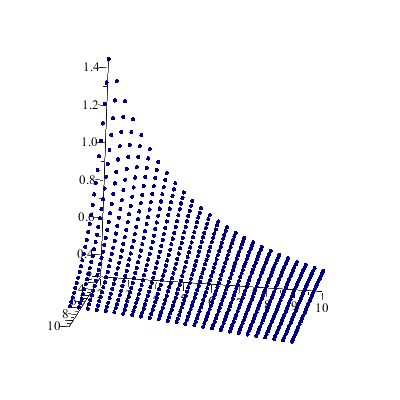
\includegraphics[width=1.3\textwidth]{doubleSimpson.png}
\caption{Simposon}
\end{figure}
\begin{figure}[H]
\centering
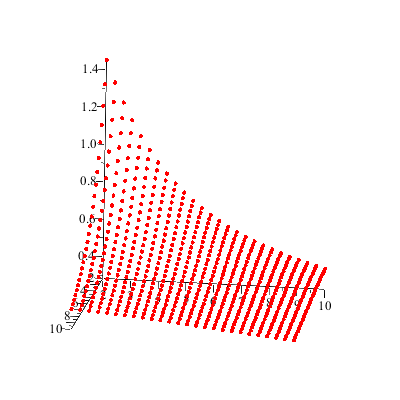
\includegraphics[width=1.3\textwidth]{doubleSimpson1.png}
\caption{Maple}
\end{figure}
从上图结合原始绘图数据可以看出两者的差别不明显,说明本题推导的二重Simpson公式还是十分有效的二重积分数值格式,在试验中发现,为避免舍入误差的影响,划分原始积分区域不应该划得太细.

\section{第四章第二题}
\subsection{问题提出及相关背景知识}
题目给出一个方程,要求用给出的两种不动点格式以及牛顿法求方程的数值解,并在理论上分析两种不动点格式是否局部收敛,以及如果收敛
收敛速度如何,最后根据实际上机结果验证理论分析的结果。
\subsection{问题理论分析及解决方案}
先推导两种不动点格式是否收敛,题目所给的两种不动点格式分别如下:
\begin{enumerate}
	\item 不动点格式1
	\[x_{k+1}=arccos(-1//(1+e^{-2x_k})),k=01,2,\cdots \]
	\item 不动点格式2
	\[x_{k+1}=0.5\ln(-1/(1+1/cosx_k))\]
\end{enumerate}
容易得出格式1与2都对应方程的一个不动点问题。然后下面证明,格式1收敛,格式2不收敛。

先证明格式1收敛,设$f(x)=arcos(-1/(1+e^{-2x}))$,则可以计算出$|f'(x)|<1,x \in (2,4)$,且$|f'(x)|\neq 0,x\in (3,3.5)$,则由不动点方法的收敛阶数推导,该方法的收敛速度为1阶的。

再证明格式2不局部收敛,另f(x)为不动点格式对应的迭代函数,计算可得$\exists x\in (2.9,3.1) st |f'(x)|>1$,于是可以说明格式2不局部收敛。

注意到在所求函数零点附近,该函数的一阶导数不为0,故对应牛顿法为2阶收敛的。
\subsection{计算成果分析}
下面列出三种格式的结果,并与其与Python的Scipy包计算的结果进行对比,做出每种方法的误差,具体内容如下:
\begin{center}
    \begin{longtable}{|c|c|c|}
        \caption{不动点格式1}\\
        \hline
        迭代次数& 相对误差\\
        \hline
        1& 0.00516545\\
        \hline
        2& 0.000336909\\
        \hline
        3& 2.19217e-05\\
        \hline
        4& 1.42615e-06\\
        \hline
        5& 9.27776e-08\\
        \hline
        6& 6.03318e-09\\
        \hline
    \end{longtable}
\end{center}
\begin{center}
    \begin{longtable}{|c|c|c|}
        \caption{不动点格式2}\\
        \hline
        迭代次数& 相对误差\\
        \hline
        1& 9.27776e-08\\
        \hline
        2& 1.42615e-06\\
        \hline
        3& 2.19217e-05\\
        \hline
        4& 0.000336909\\
        \hline
        5& 0.00516545\\
        \hline
        6& 0.0764212\\
        \hline        
    \end{longtable}
\end{center}
\begin{center}
    \begin{longtable}{|c|c|c|}
        \caption{牛顿法}\\
        \hline
        迭代次数& 相对误差\\
        \hline
        1& 3.07642\\
        \hline
        2& 0.0210937\\
        \hline
        3& 0.00268953\\
        \hline
        4& 5.63034e-05\\
        \hline
        5& 2.57304e-08\\
        \hline
        6& 2.75335e-12\\
        \hline
    \end{longtable}
\end{center}
由上计算结果可以看出,不动点格式1为局部收敛的,不动点格式2不收敛。在收敛速度方面,牛顿法在第六步的精度已经达到$10^{-12}$,而不动点格式1只有$10^{-9}$。这两个特点均与我们的理论分析相符。
\subsection{本次上机反思}
在本题中两个不动点收敛格式,格式1与格式2均是与原方程完全等价的不动点问题,但是两个方法的收敛性质完全不同。我们在平时设计不动点格式的时候
必须从理论上考虑到这种方法的收敛性与收敛速度。
\section{第四章第三题}
\subsection{问题提出及相关背景知识}
题目要求用牛顿法与Broyden方法求一个方程组的数值解.
\subsection{问题理论分析及解决方案}
容易看出题目的精确解为$x=(0,1)^T$,可以将所获得的计算结果与该解对比,得到两种方法的收敛速度的对比。在编制程序的时候,引入向量的二范数$\|\cdot \|_2$,并将$\|x_k-x_{k-1}\|_2<\epsilon$作为迭代终止的条件。


\subsection{计算成果分析}
下面列出两种方法的计算成果,如下:
\begin{center}
    \begin{longtable}{|c|c|c|}
        \caption{牛顿法结果} \\
        \hline
        迭代次数& 误差 \\
        \hline
        1& 1 \\
        \hline
        2& 0.0833817 \\
        \hline
        3& 0.000297755 \\
        \hline
        4& 2.33422e-08 \\
        \hline
        5& 9.4437e-17 \\
        \hline
        6& 9.4437e-17 \\
        \hline
    \end{longtable}
\end{center}
\begin{center}
    \begin{longtable}{|c|c|c|}
        \caption{Broyden算法结果} \\
        \hline
        迭代次数& 误差 \\
        \hline
        1& 0.0833817\\
        \hline
        2& 0.000633597 \\
        \hline
        3& 0.000310409 \\
        \hline
        4& 5.44241e-05 \\
        \hline
        5& 1.78089e-07 \\
        \hline
        6& 7.19784e-10 \\
        \hline
        7& 2.22499e-12 \\
        \hline
        8& 1.35593e-15 \\
        \hline
        9& 1.44847e-16 \\
        \hline
        10& 1.82564e-16 \\
        \hline
    \end{longtable}
\end{center}

由上面的计算结果可以看出,牛顿法在第五步已经达到了机器精度。而Broyden算法在第九步达到了机器精度。于是牛顿法的收敛速度
高于Broyden算法,这一点与理论分析相合(理论上牛顿法为2阶收敛,而Broyden算法为超线性收敛)。
\subsection{本次上机反思}
虽然从上面结果看出来,牛顿法计算效果远远好于Broyden算法。但是本题方程的阶数较低(2阶),两种方法的计算速度没有体现出明显差别,
如果以后在实际问题中遇到阶数较高的情况,此时,牛顿法的计算时间复杂度太高,就要在两种方法做一个选择。
\section{第四章第四题}
\subsection{问题提出及其相关背景}
\subsection{计算成果分析}
\subsection{上机反思}
\end{document}


